\chapter{Development of a Proxy for Google Cloud Storage}

\section{Context}
\acf{CI} pipelines automatically generate numerous artifacts such as tests, code coverage and \ac{VRT} reports. These artifacts are essential for validating software quality and approving \acs{PR} throughout the development lifecycle.

Initially, some of these reports were stored using GitHub Actions Artifacts. Although this solution integrates naturally with GitHub workflows, it presents several limitations. The storage consumed by artifacts continuously increases over time, especially for large visual regression reports, leading to higher infrastructure costs. Moreover, GitHub artifacts cannot be accessed directly through a web browser. Developers must download the archive, extract its contents, and open the report locally before consulting it.

To overcome these limitations, Rakuten France decided to migrate \ac{CI} artifacts (\ac{VRT} reports) to private \acf{GCS} buckets. \ac{GCS} provides scalable, durable and cost-effective object storage. However, because the buckets remain private, reports cannot be accessed without Google Cloud authentication.

To provide secure yet transparent access to these reports, a proxy application was developed. The application authenticates against Google Cloud Storage on behalf of internal users and exposes reports through \acs{HTTP} endpoints while keeping the storage infrastructure completely private.

\section{Objectives}

The project pursued both technical and educational objectives, including:

\begin{itemize}
\item Keep Google Cloud Storage buckets private and secure.
\item Allow internal access to reports through a Rakuten web application.
\item Simplify report consultation directly from a browser.
\item Provide report discovery, verification and download features.
\item Discover the complete software lifecycle from requirements analysis to deployment and maintenance.
\end{itemize}

\section{System Architecture}

The application follows a proxy architecture. Every request is received by the proxy instead of directly reaching Google Cloud Storage.

\begin{figure}[H]
\centering
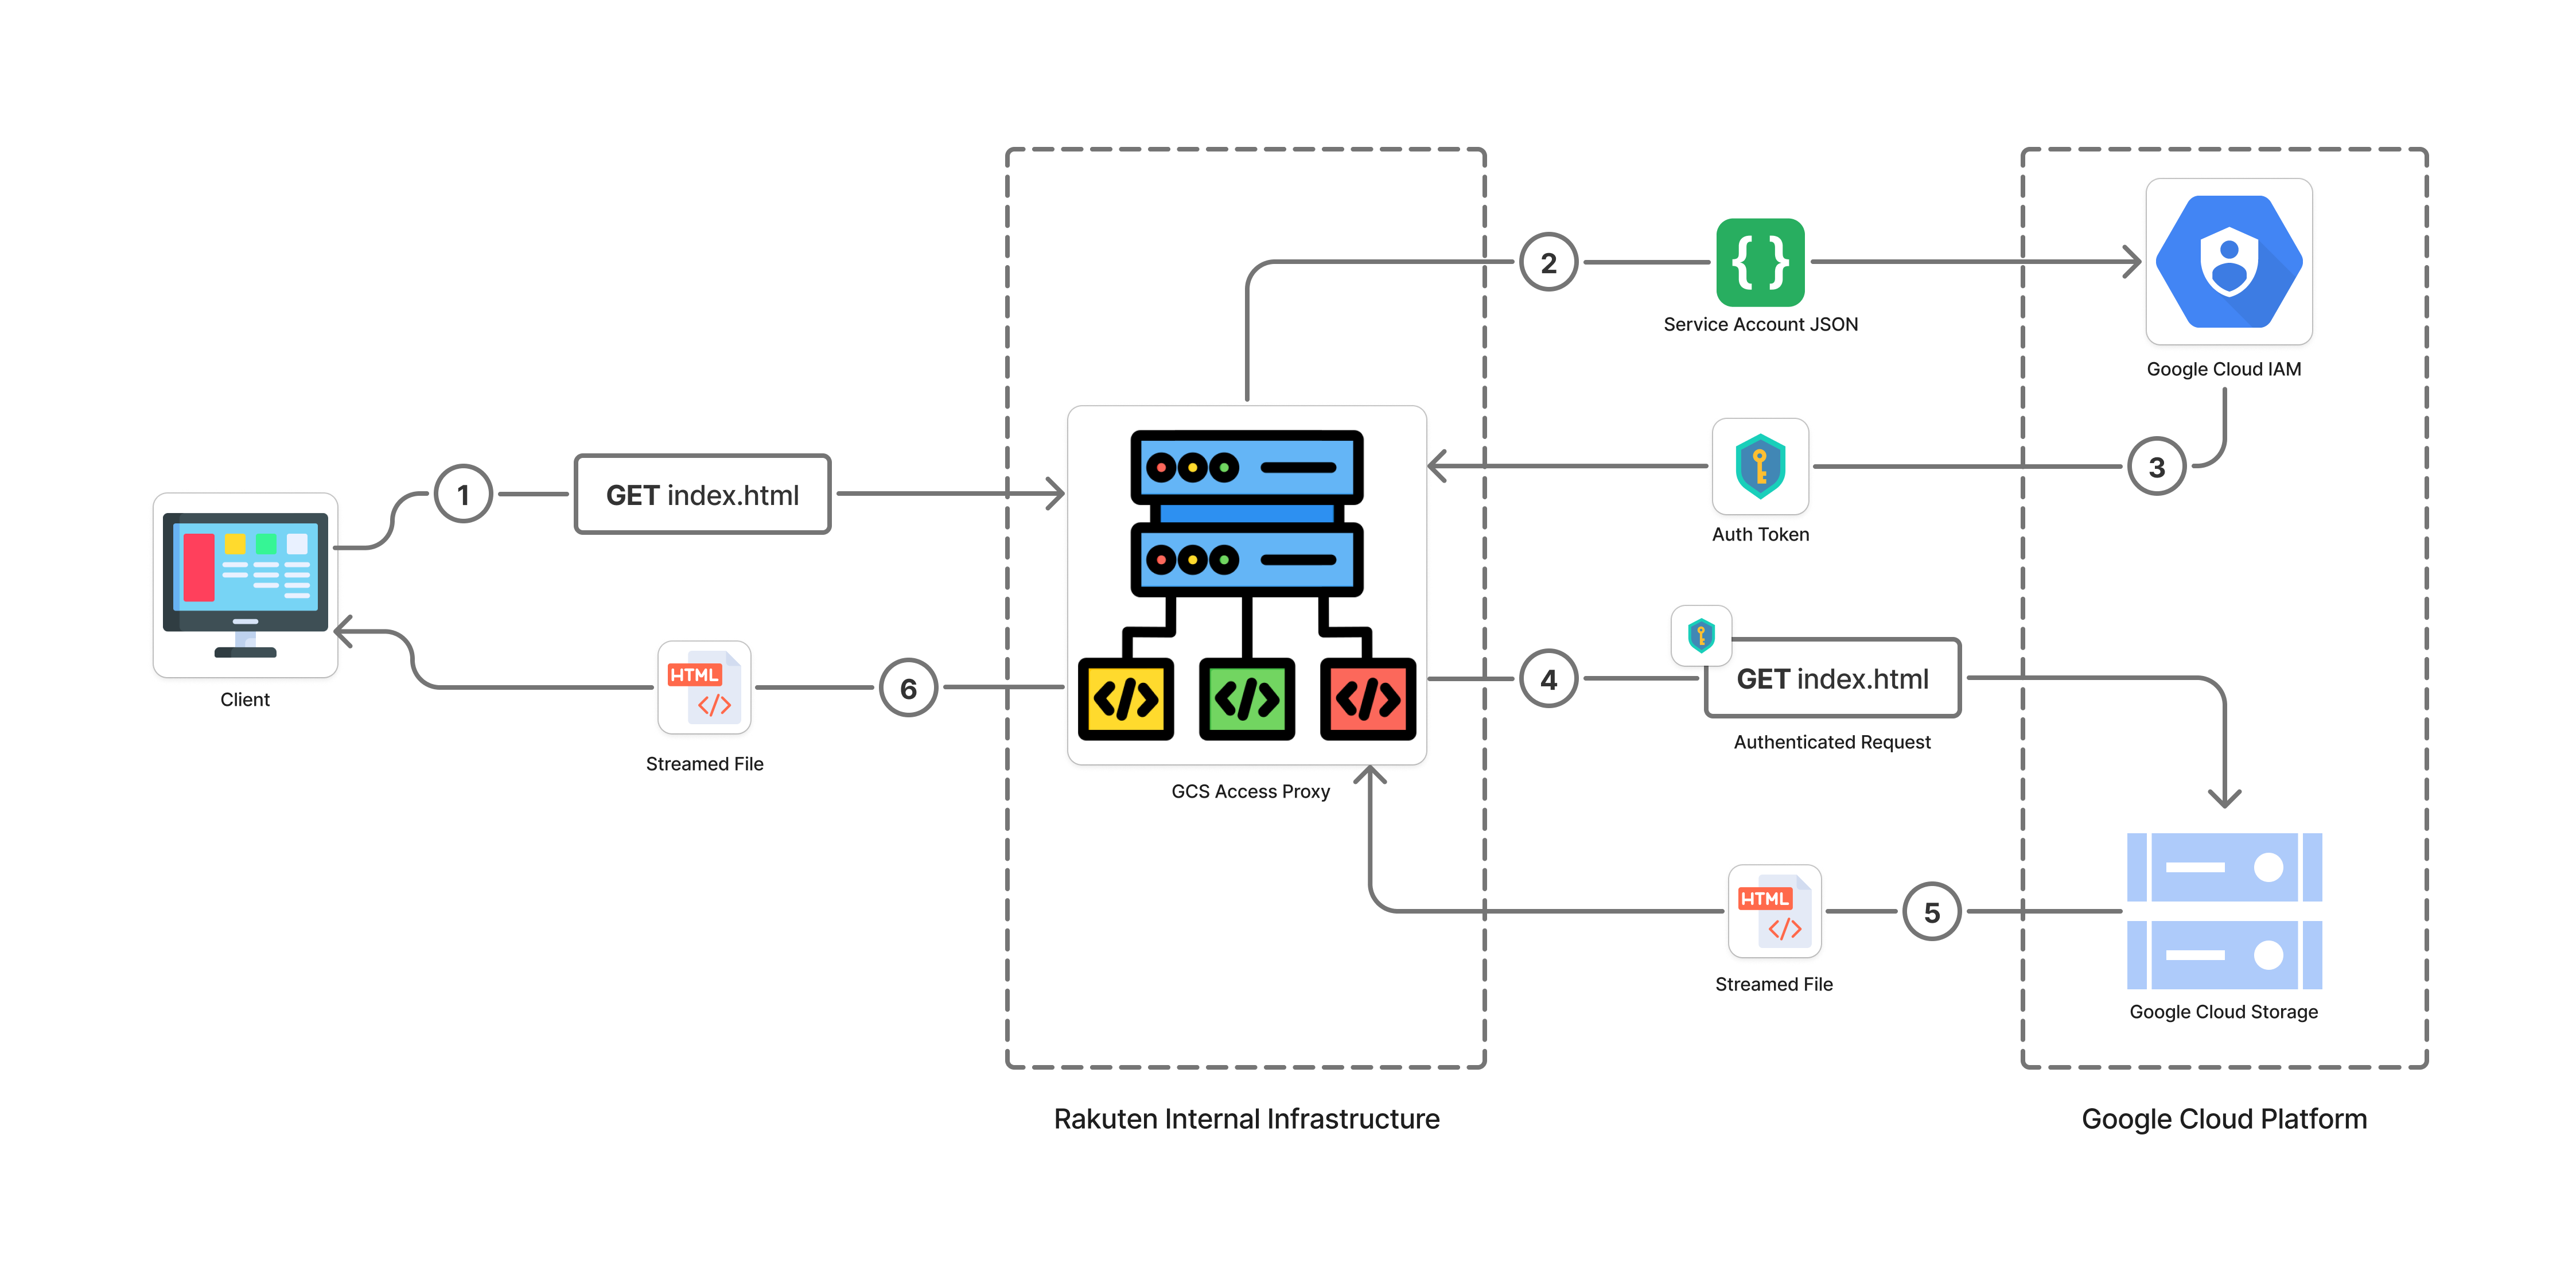
\includegraphics[width=.95\textwidth]{../assets/ci_reports_gcs_access/gcs_proxy_architecture.png}
\caption{Overall architecture of the proxy.}
\label{fig:gcs_architecture}
\end{figure}

The processing workflow is summarized below:

\begin{enumerate}
\item Receive an incoming HTTP request.
\item Extract the bucket name and object path.
\item Authenticate using a Google Cloud Service Account.
\item Cache the auth token for a specific amount of time.
\item Request the object through the Google Cloud Storage API.
\item Stream the object directly to the client.
\item Return the corresponding HTTP response.
\end{enumerate}

\section{Authentication and Token Caching}

The Infrastructure team provides the application with a Google Cloud Service Account JSON credential. During startup, the application loads these credentials and generates an authentication access token.

Since generating a token for every request would introduce unnecessary latency, the application stores the generated token in memory until its expiration time (e.g., 1 hour). When the token expires, a new one is automatically generated and replaces the previous token. This caching strategy significantly reduces authentication overhead under heavy workloads.

\section{Streaming Mechanism}

Instead of downloading the complete object before sending it to the client, the application streams files directly from Google Cloud Storage to the HTTP response. Streaming reduces memory consumption, decreases latency, and allows very large HTML reports and visual regression artifacts to be served efficiently.

\section{Technology Stack}

The project is developed using \acs{TS} as the primary programming language, with Node.js as the runtime environment and pnpm as the package manager. The HTTP server is implemented using the \textbf{Hono} framework, a lightweight and high-performance web framework designed for building modern HTTP servers and APIs with \acs{JS} and \acs{TS}.

\textbf{Hono} is based on Web Standard APIs, enabling applications to run across multiple runtimes such as Node.js, Bun, Deno, and Cloudflare Workers. It also provides a simple Express-like routing system while maintaining a minimal footprint.

The web interface of the application is developed using standard web technologies, including \acs{HTML}, \acs{CSS}, and \acs{JS}.
 
\acf{GCS} Google Cloud Storage is used as the storage solution for hosting \ac{CI}-generated artifacts, while Google Cloud Service Account credentials provide secure and controlled authentication for accessing cloud resources.

The rest of the project version control, \ac{CI}/\acs{CD} pipelines and maintenance are managed by the internal DevOps tools presented in section~\ref{sec:rakuten-devops-tools}.

\section{\acs{API} Endpoints}

The application exposes several REST endpoints that can be classified into two categories: functional endpoints and operational endpoints.

\subsection{Functional Endpoints}

The basic endpoint structure is defined as follows:

\[
\texttt{<Operation>/<Bucket\ name>/<FilePath>}
\]

where the \texttt{FilePath} parameter can represent either a direct file name
or a nested path pointing to a file or folder within the specified bucket.

Concretely, the application provides the following endpoints:

\begin{itemize}
    \item \texttt{GET /gcs/<bucket>/<filePath>}: Serve a file (or a report index.html file) directly from \acf{GCS}.
    \item \texttt{GET /download/<bucket>/<filePath>}: Download a report or a set of files as a ZIP archive.
    \item \texttt{GET /check-exist/<bucket>/<filePath>}: Verify whether a specific report or file exists.
    \item \texttt{GET /search/<bucket>/<filePath>}: Search for the latest report matching a given prefix or suffix.
    \item \texttt{GET /buckets}: List all accessible Google Cloud Storage buckets.
\end{itemize}

\subsection{Operational Endpoints}

The application provides also a set of several operational endpoints to facilitate use, monitoring and maintenance.

\paragraph{Web Interface}

A lightweight web interface available at \texttt{/} allows users to execute supported operations without manually constructing HTTP requests.

Figures~\ref{fig:file_existence_check}  illustrate the web interface (in light mode) for checking the existence of a report file while figure~\ref{fig:file_non_existence_check} illustrates the web interface (in dark mode) for checking the non-existence of a report file.

\begin{figure}[H]
\centering
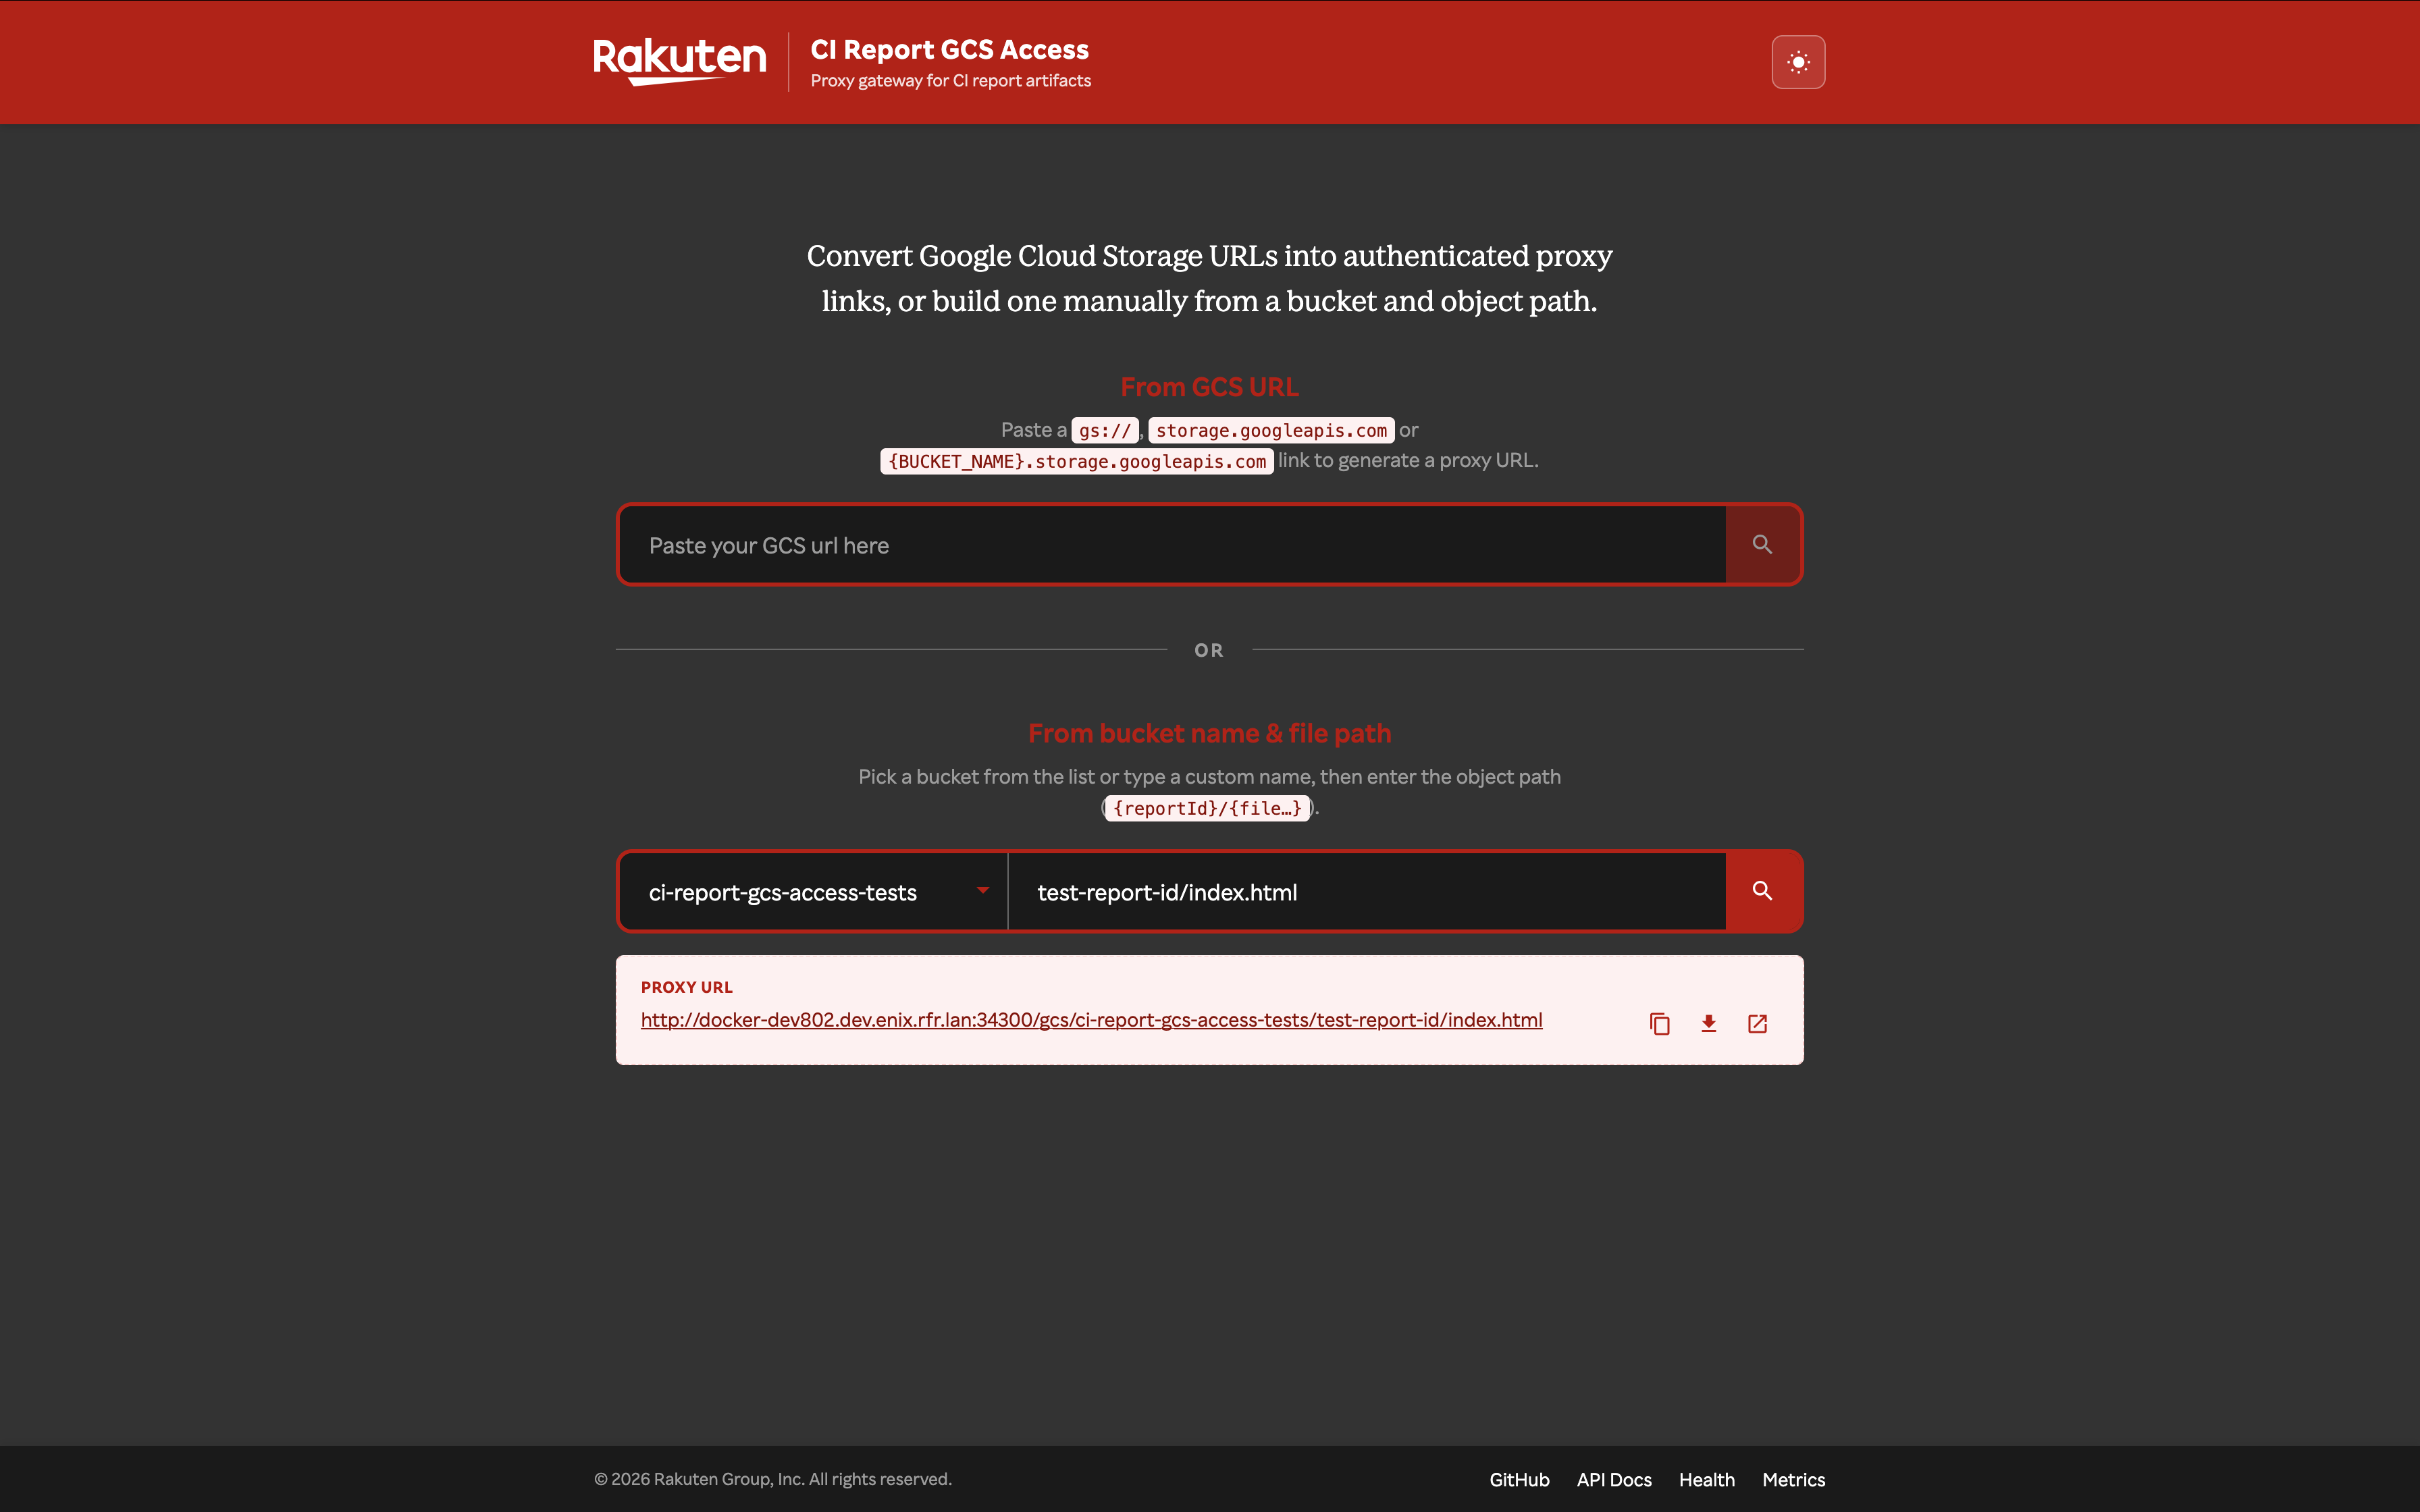
\includegraphics[width=.9\textwidth]{../assets/ci_reports_gcs_access/file_exist_dark.png}
\caption{Web interface for checking the existence of a report file.}
\label{fig:file_existence_check}
\end{figure}

\begin{figure}[H]
\centering
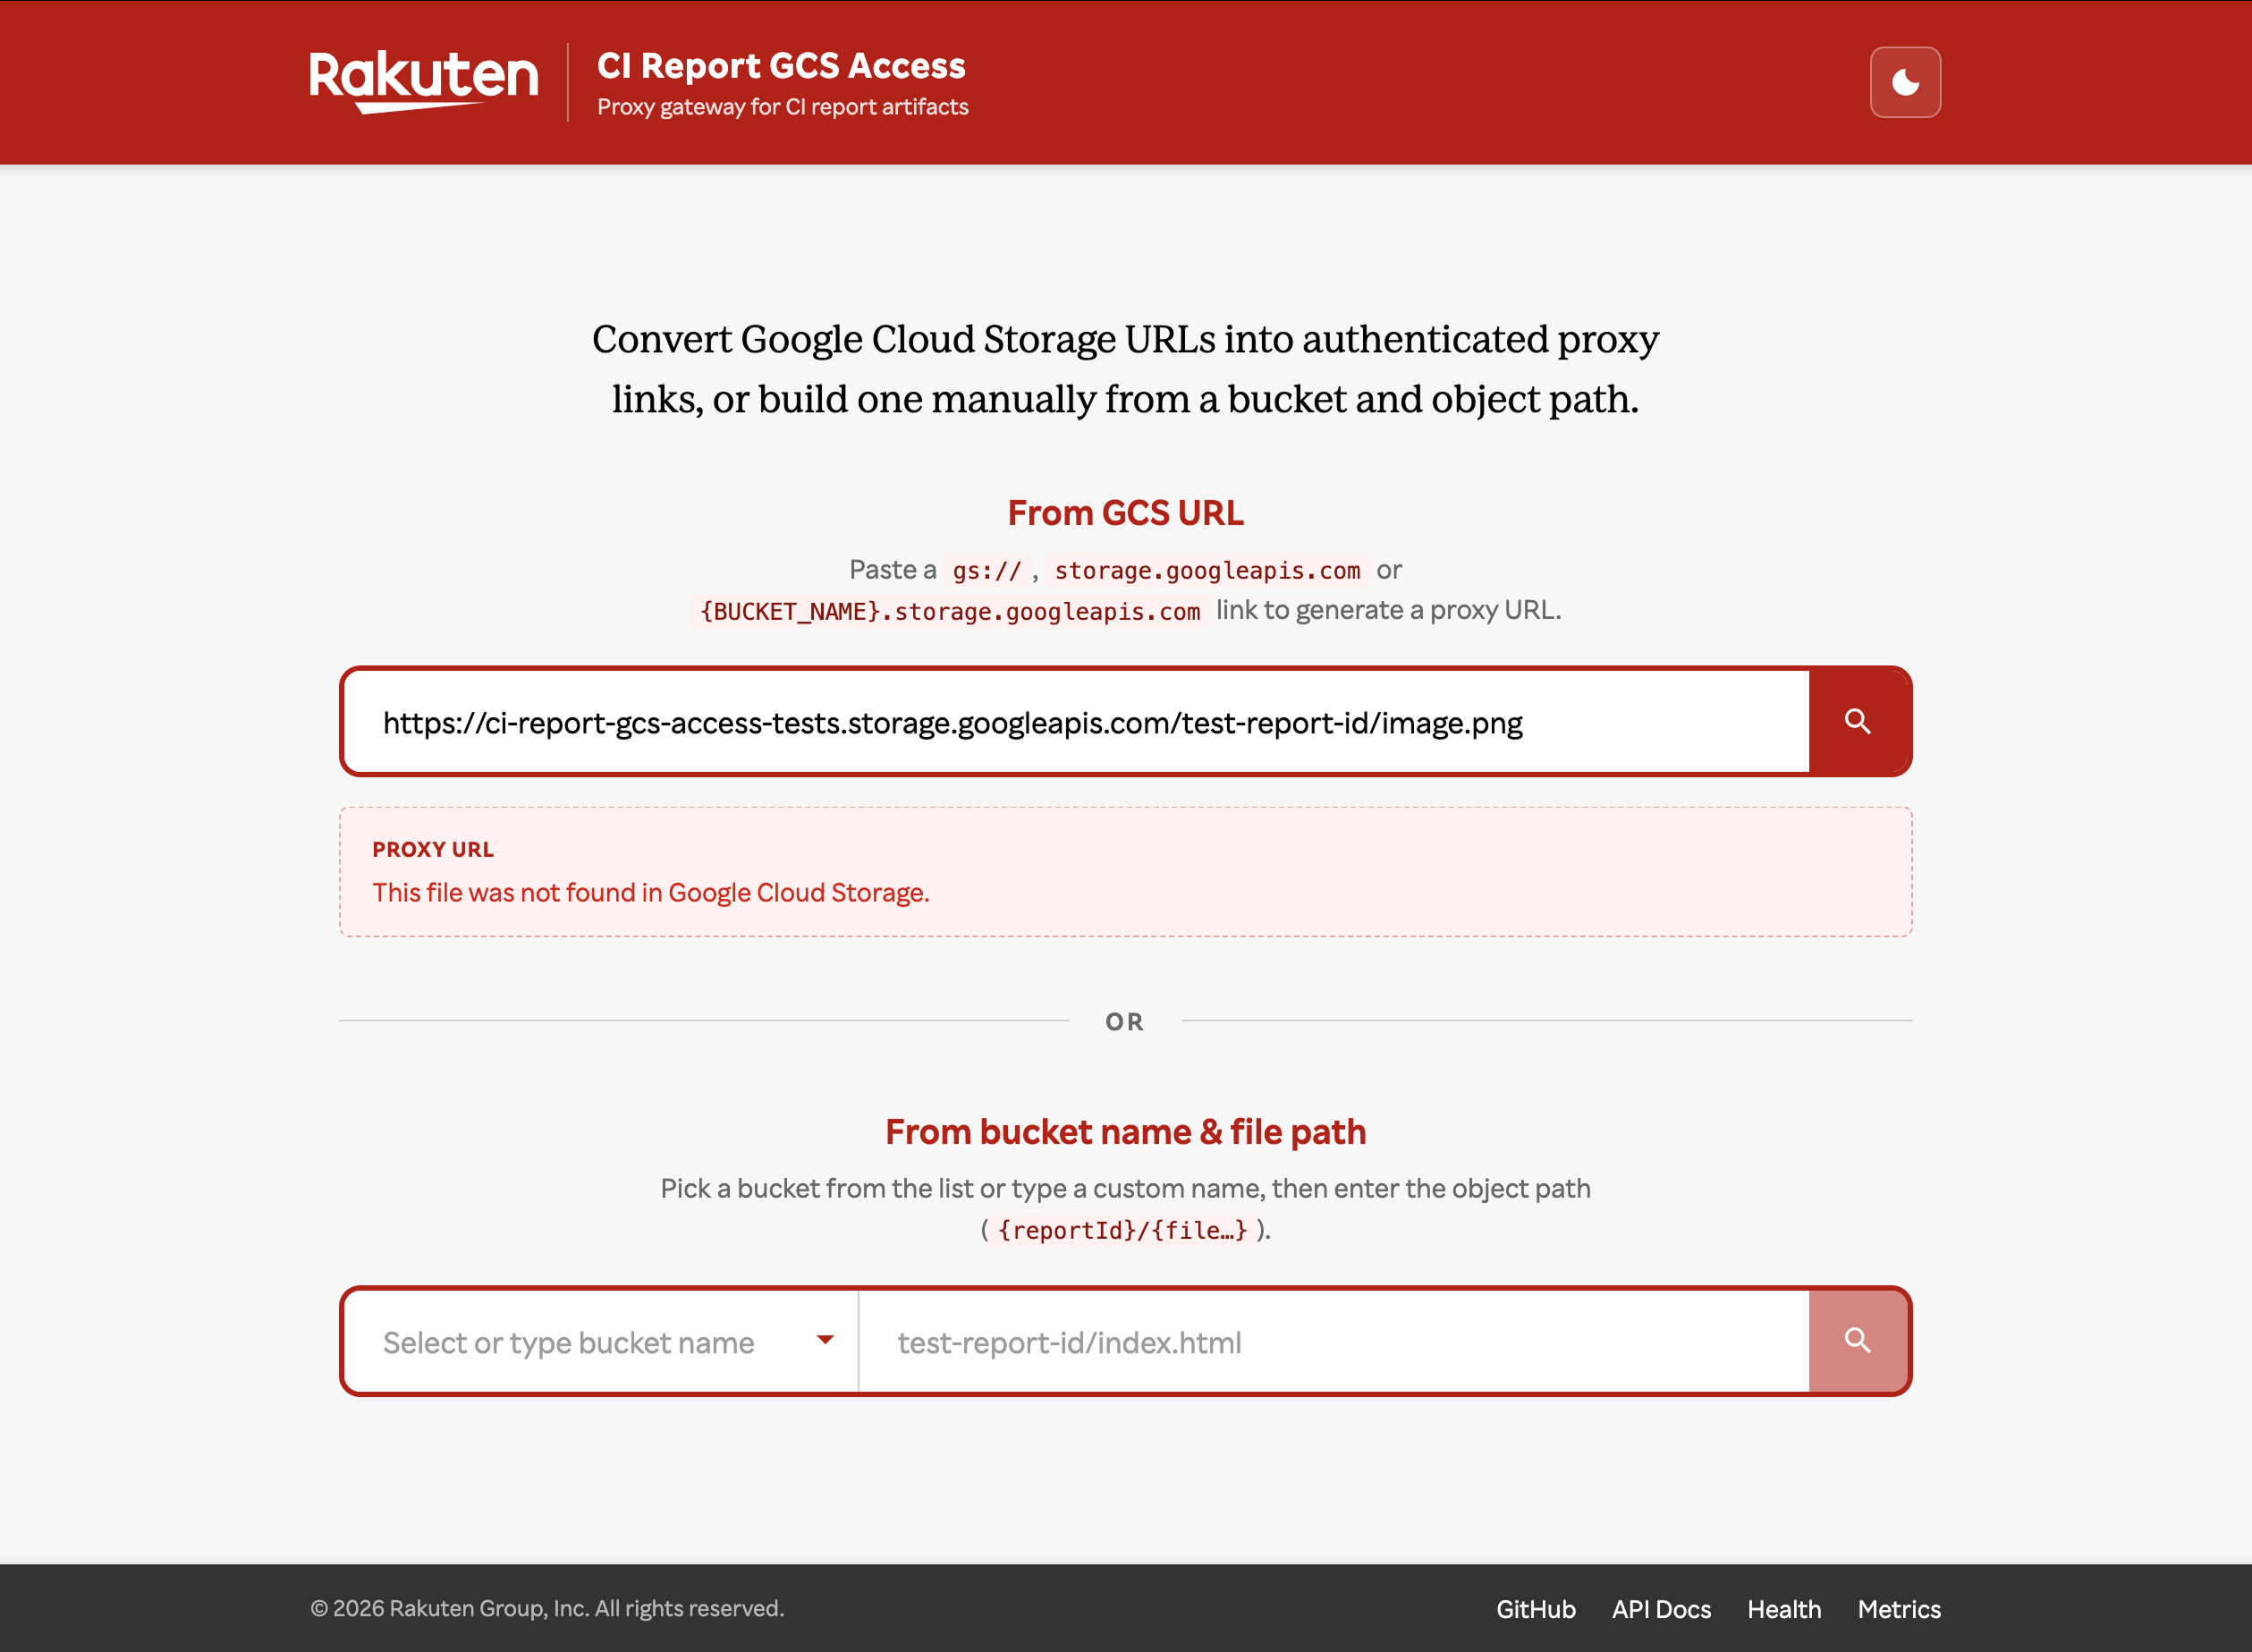
\includegraphics[width=.9\textwidth]{../assets/ci_reports_gcs_access/file_not_exist_light.png}
\caption{Web interface for checking the non-existence of a report file.}
\label{fig:file_non_existence_check}
\end{figure}

\paragraph{Health Check}

The /health endpoint is used by Consul to verify the availability of the service. The Consul agent periodically (e.g., every 5 seconds) sends a request to this endpoint, which returns a \acs{JSON} object containing a \texttt{status} key with one of three possible values: \textcolor{green}{\texttt{UP}}, \textcolor{red}{\texttt{DOWN}}, or \textcolor{orange}{\texttt{DEGRADED}}. Based on this status, Consul determines the health of the service and can trigger alerts or take corrective actions when necessary.

Figure~\ref{fig:consul_health_check} illustrates the health check of the deployed application on Consul.

\begin{figure}[H]
\centering
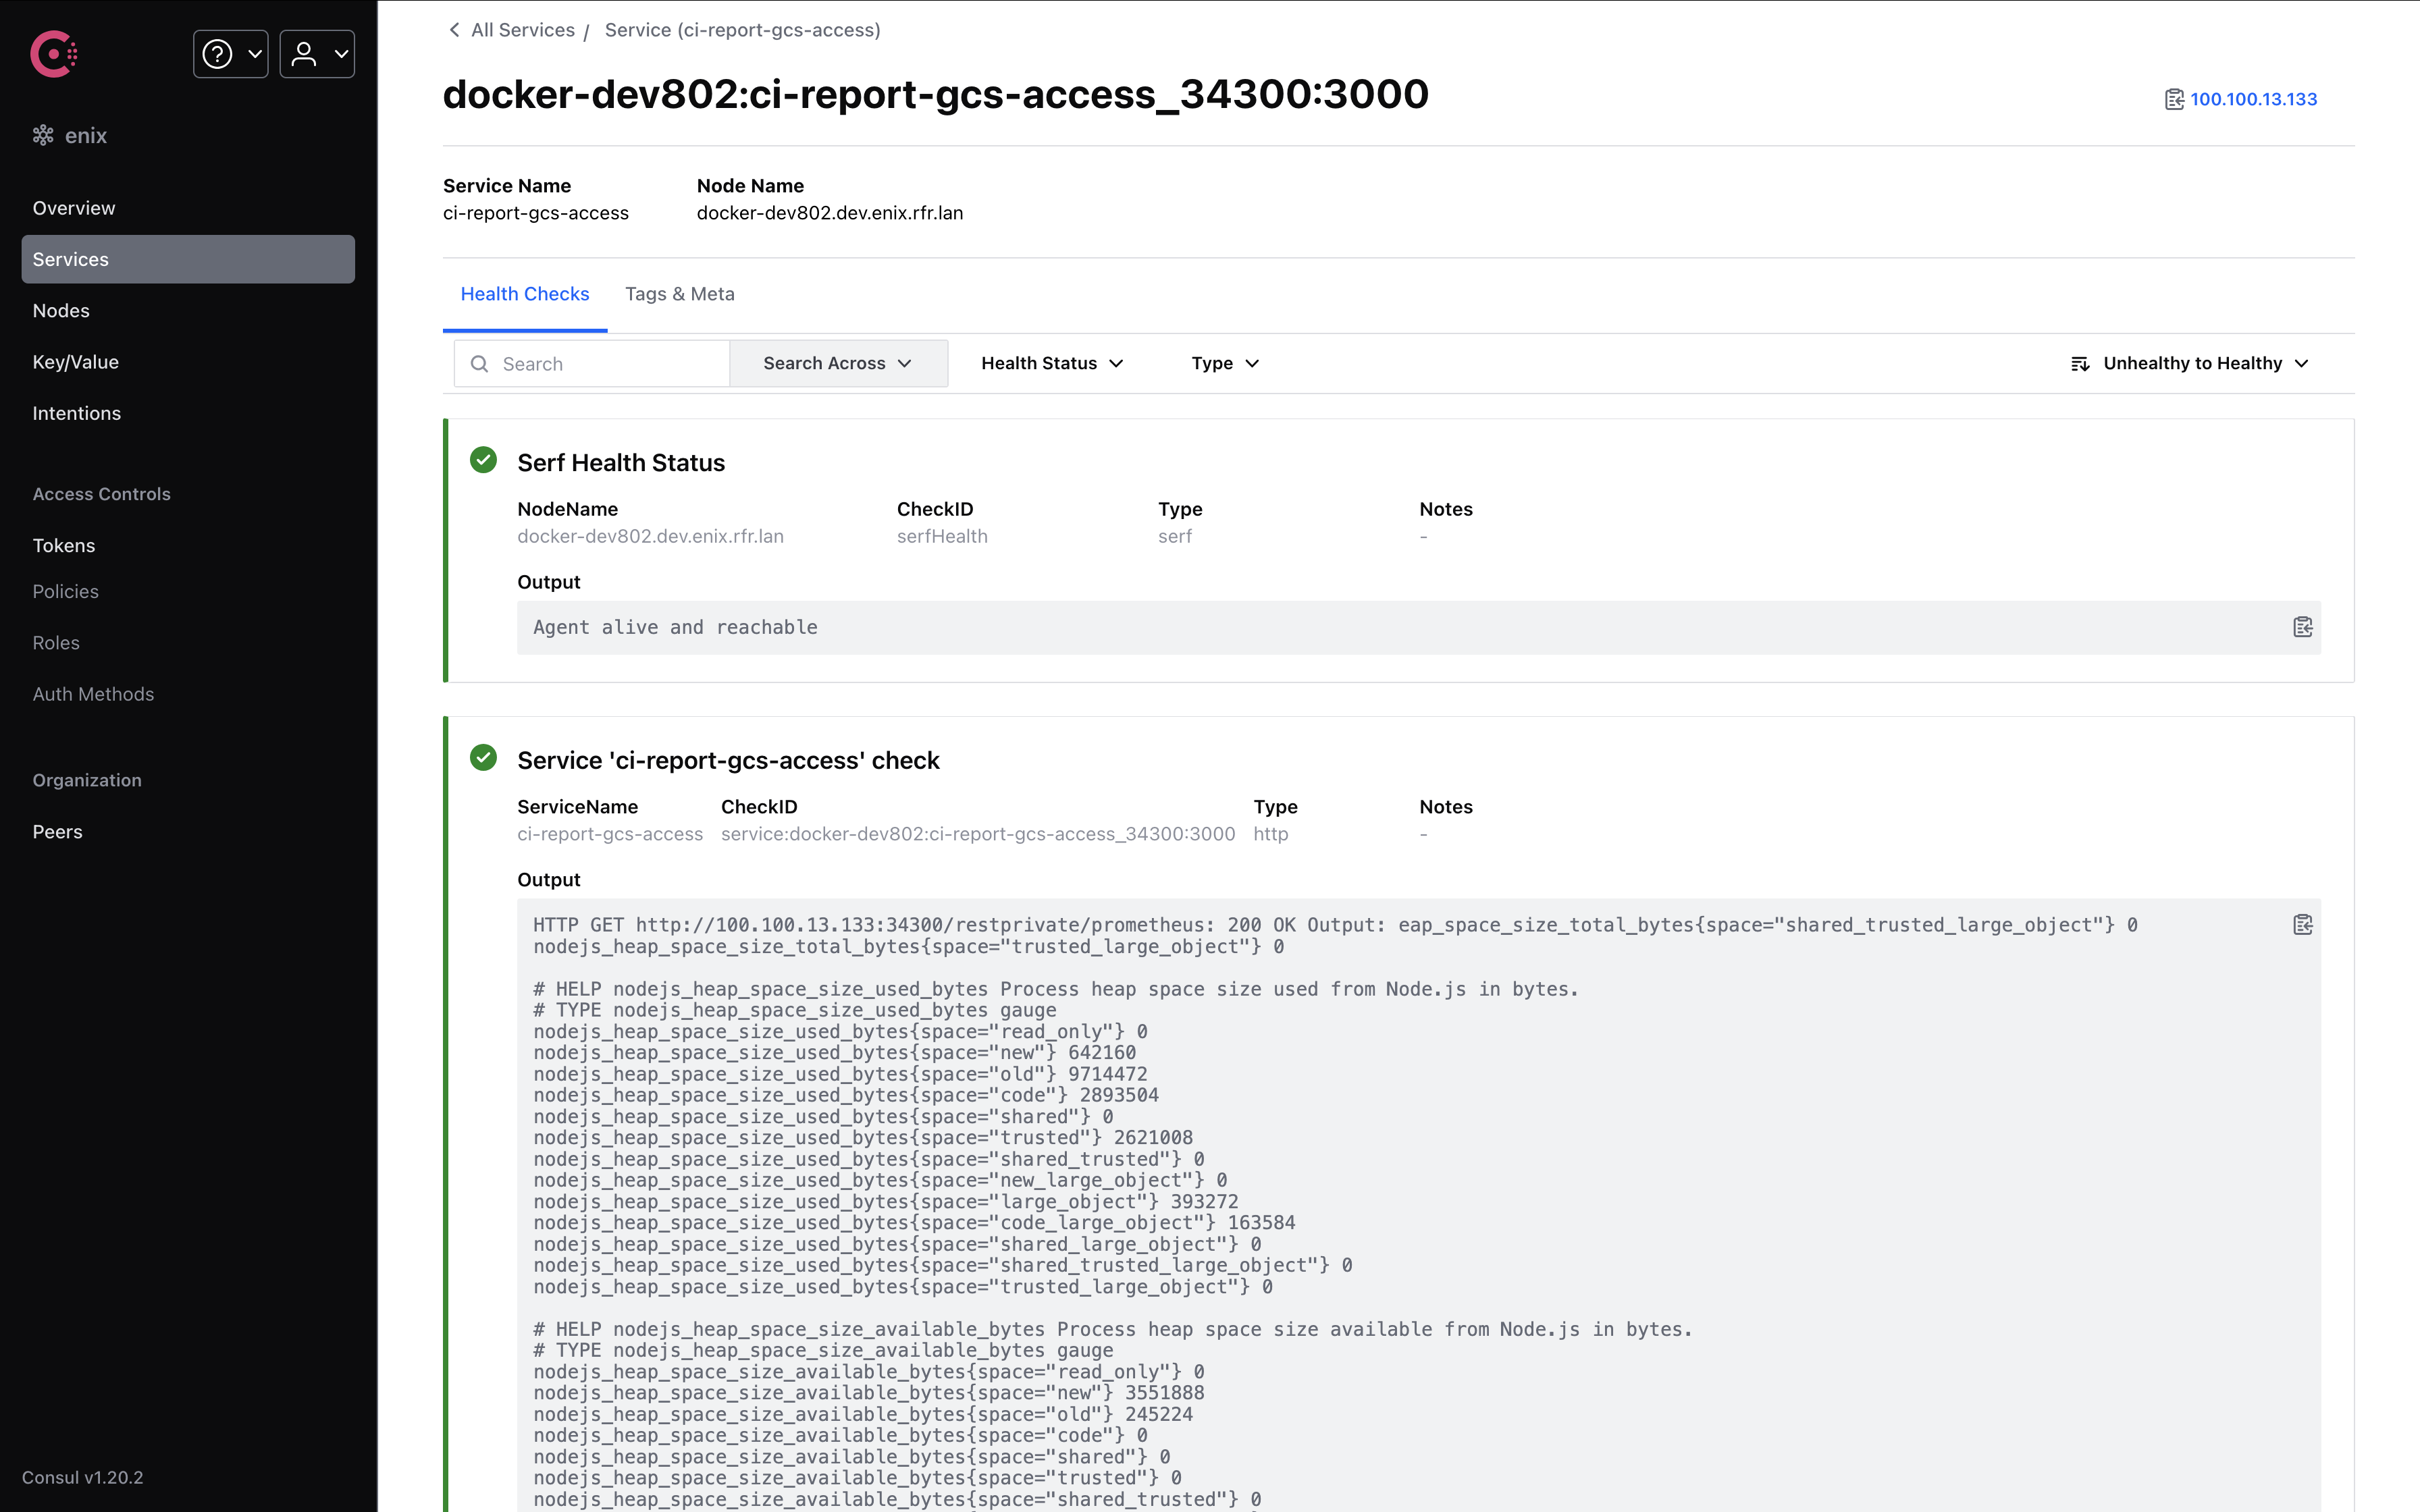
\includegraphics[width=.95\textwidth]{../assets/ci_reports_gcs_access/consul_health_check.png}
\caption{The Proxy Health check on Consul}
\label{fig:consul_health_check}
\end{figure}

\paragraph{Metrics}

This endpoint exposes application metrics in a Prometheus-compatible format, including request counts, response times and other relevant indicators. These metrics can be collected by Prometheus and visualized through Grafana, providing valuable insights into the application's performance, availability, and overall health.

Figure~\ref{fig:metrics_exposure} shows the metrics exposed by the deployed application and accessible through the \href{https://chromewebstore.google.com/detail/prometheus-viewer/cbemcojgcihplgfjjdoplpfjmamiikcn}{Prometheus Viewer} Chrome extension.

\begin{figure}[H]
\centering
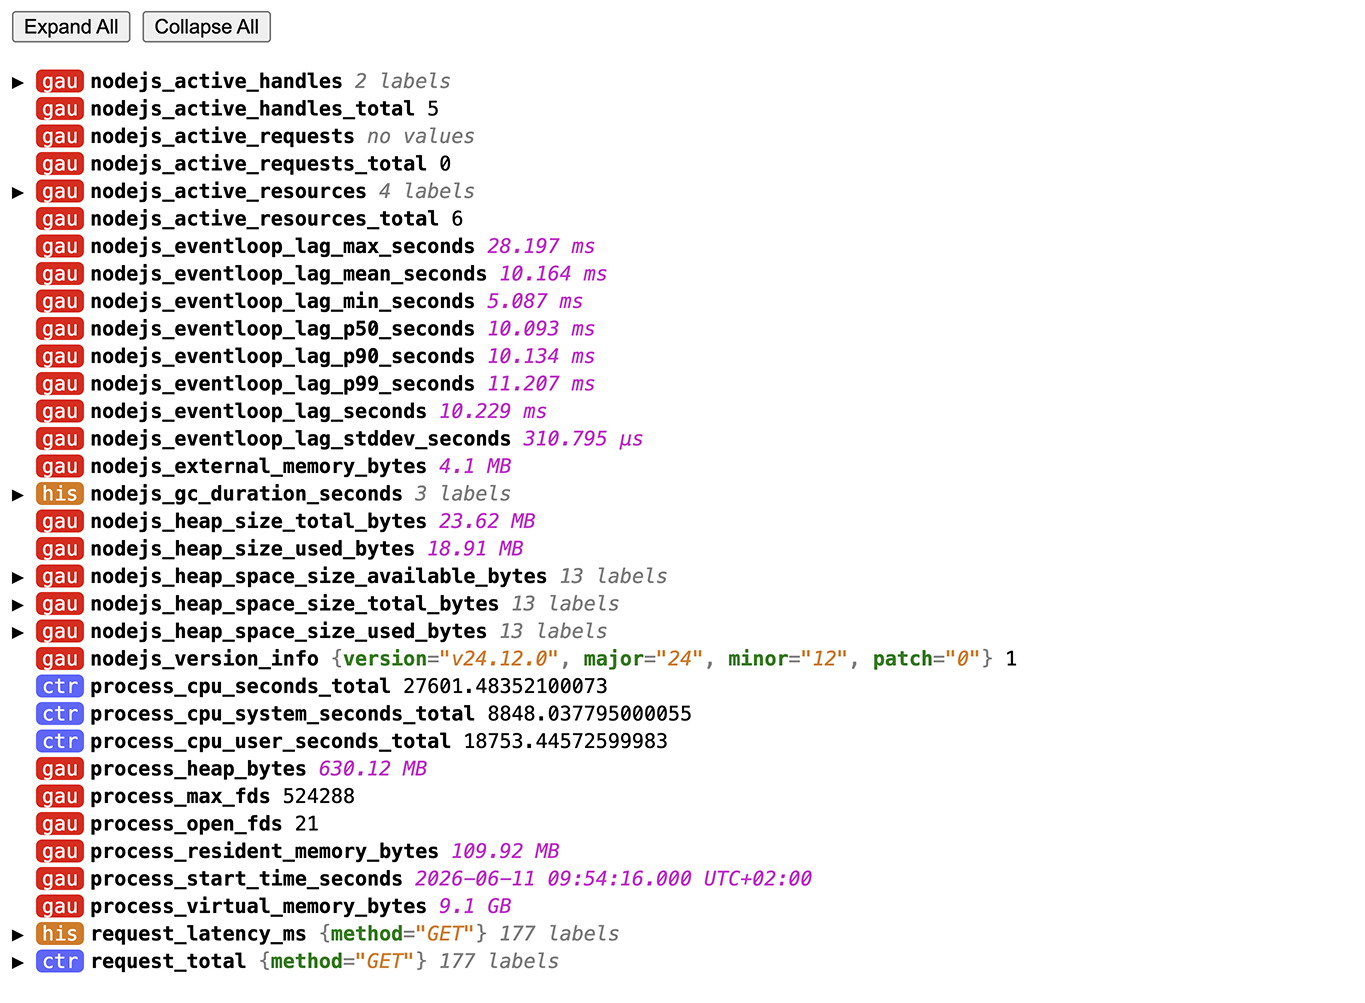
\includegraphics[width=.95\textwidth]{../assets/ci_reports_gcs_access/metrics_exposure.png}
\caption{The Proxy Metrics Exposure}
\label{fig:metrics_exposure}
\end{figure}

\paragraph{API Documentation}

Interactive API documentation is generated and exposed through Swagger/OpenAPI. Figure~\ref{fig:openapi_documentation} shows the Swagger UI interface for the proxy.

\begin{figure}[H]
\centering
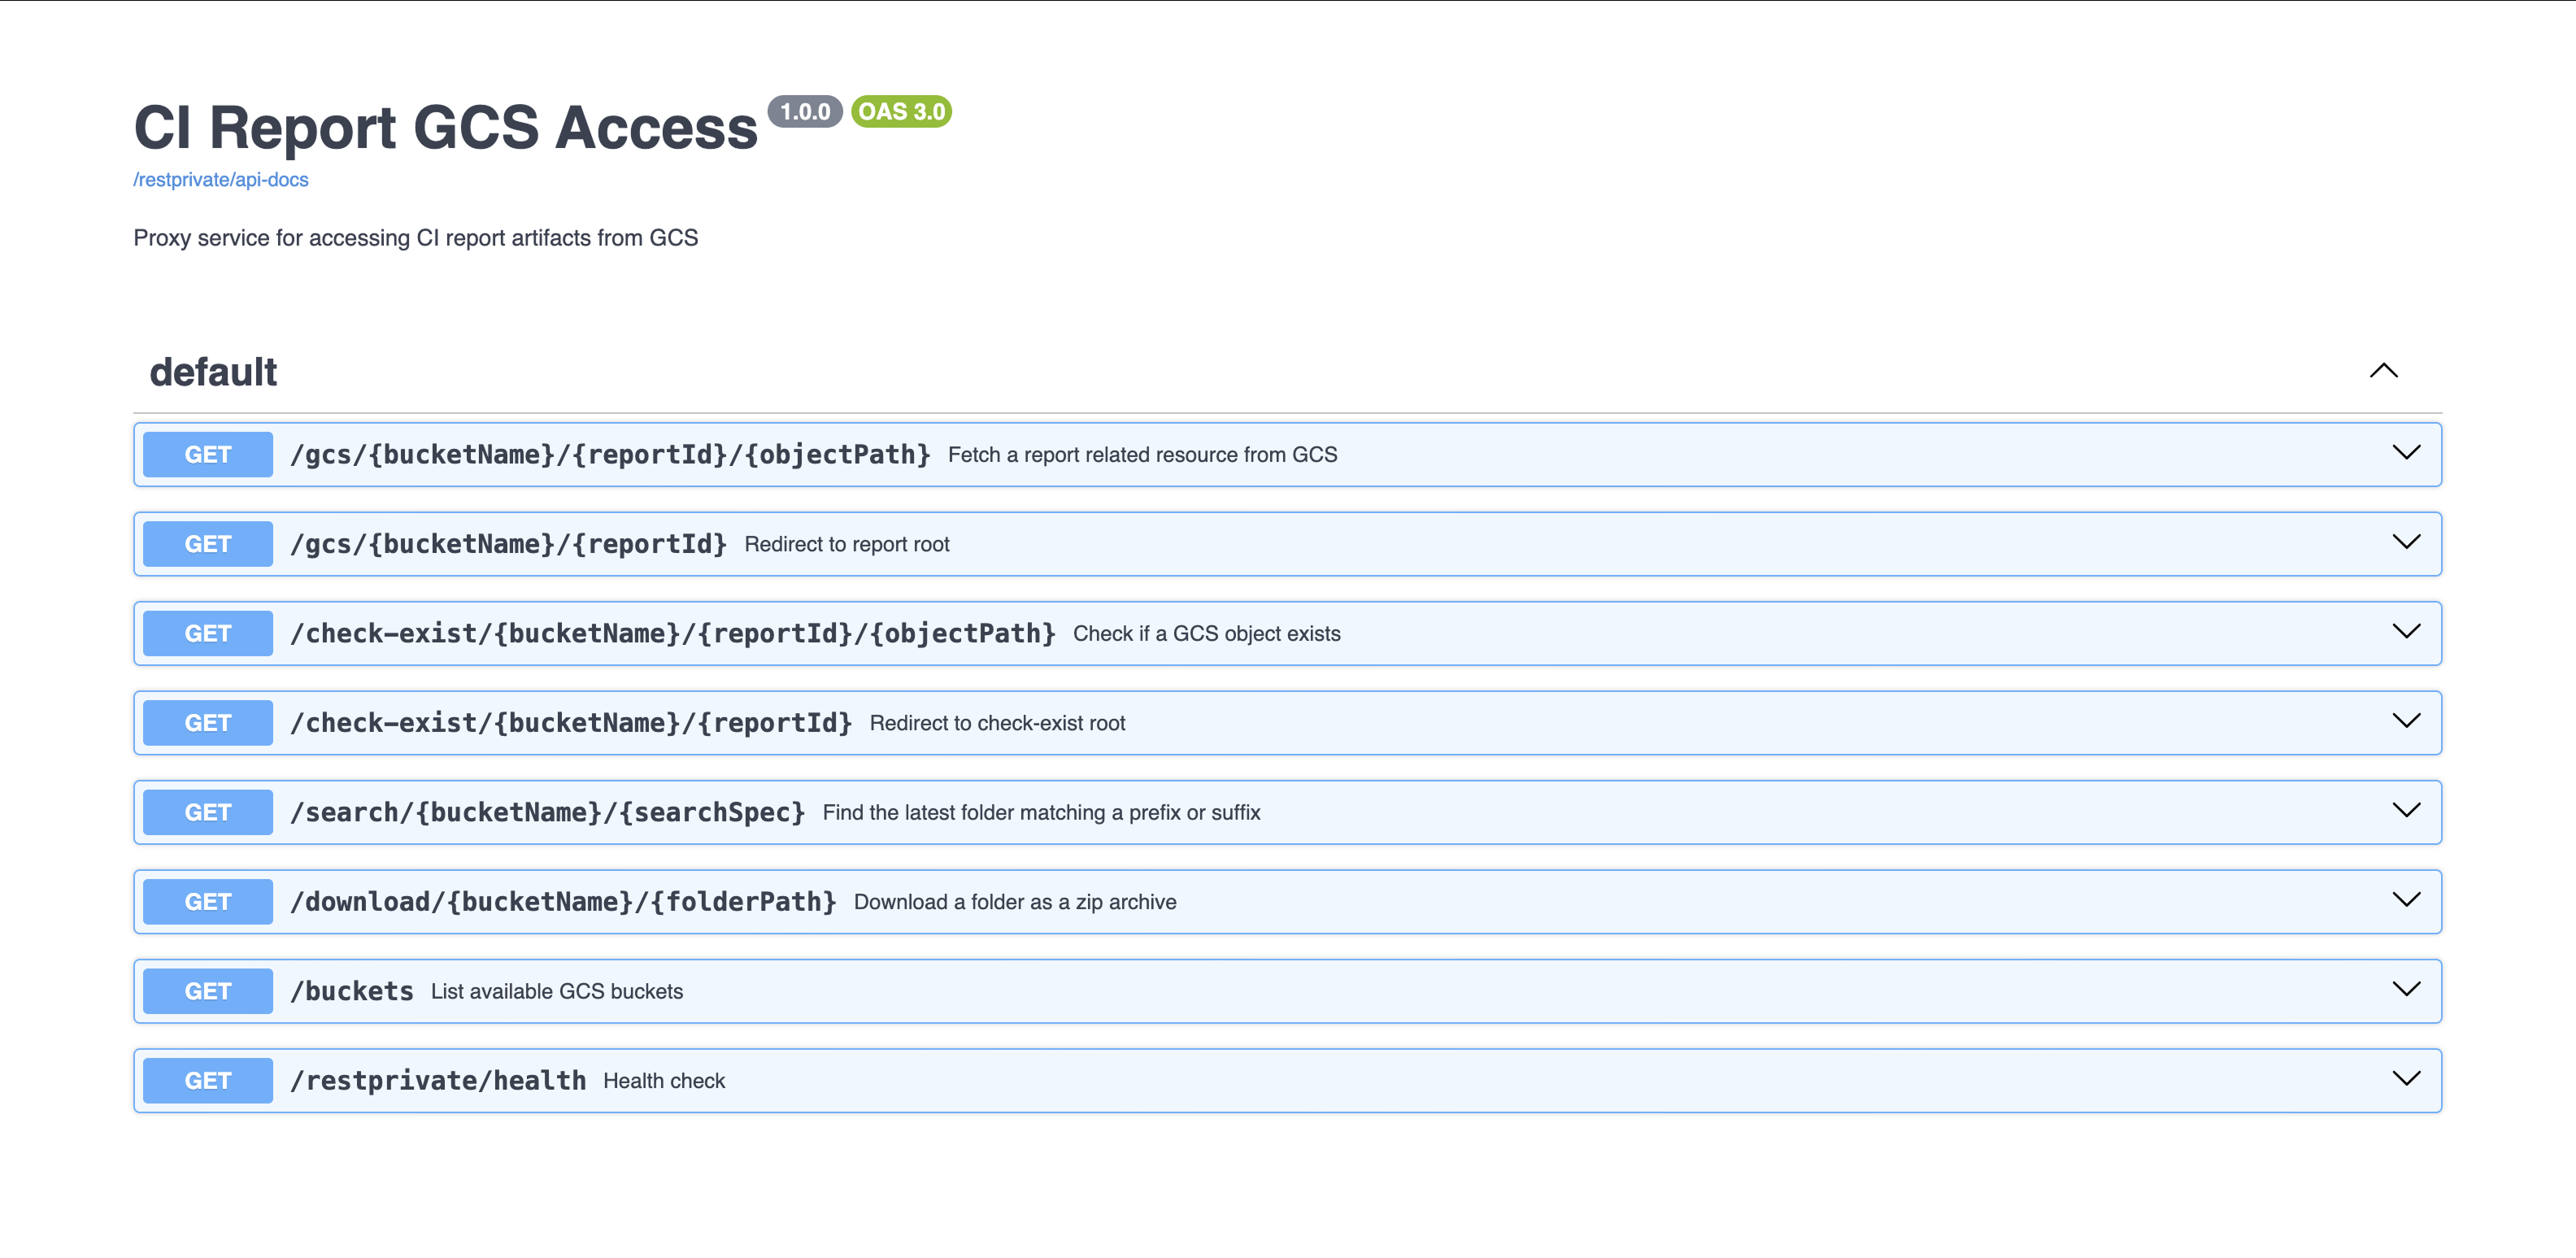
\includegraphics[width=.95\textwidth]{../assets/ci_reports_gcs_access/openapi_documentation.png}
\caption{Interactive API Swagger UI Documentation}
\label{fig:openapi_documentation}
\end{figure}

\section{Testing}

A dedicated Google Cloud Storage bucket was created for integration testing.

The test suite validates:

\begin{itemize}
  \item Serves \texttt{index.html} with correct status, content-type, and body
  \item Serves \texttt{index.html} when the report root URL has a trailing slash
  \item Serves \texttt{index.json} with correct status, content-type, and body
  \item Returns the latest matching folder for a given prefix
  \item Returns an empty folder when no prefix match is found
  \item Returns the latest matching folder for a given suffix
  \item Returns an empty folder when no suffix match is found
  \item Rejects search paths that do not use \texttt{prefix=} or \texttt{suffix=}
  \item Lists available GCS buckets
  \item Rejects file upload paths containing traversal
  \item Rejects empty file upload bodies
  \item Rejects invalid folder upload zip bodies
\end{itemize}

Load tests were also performed to verify the effectiveness of the authentication token caching mechanism. In particular, these tests aimed to confirm that cached authentication tokens are correctly reused across successive requests, thereby reducing the number of OAuth authentication requests while maintaining low response times under load.

Figure~\ref{fig:proxy-load-test} presents the result of retrieving the \texttt{index.html} file during the proxy load test. The results demonstrate the proxy's ability to handle concurrent requests while reusing cached authentication tokens, thereby reducing the need for repeated OAuth authentication requests and maintaining low response times.

\begin{figure}[H]
    \centering
    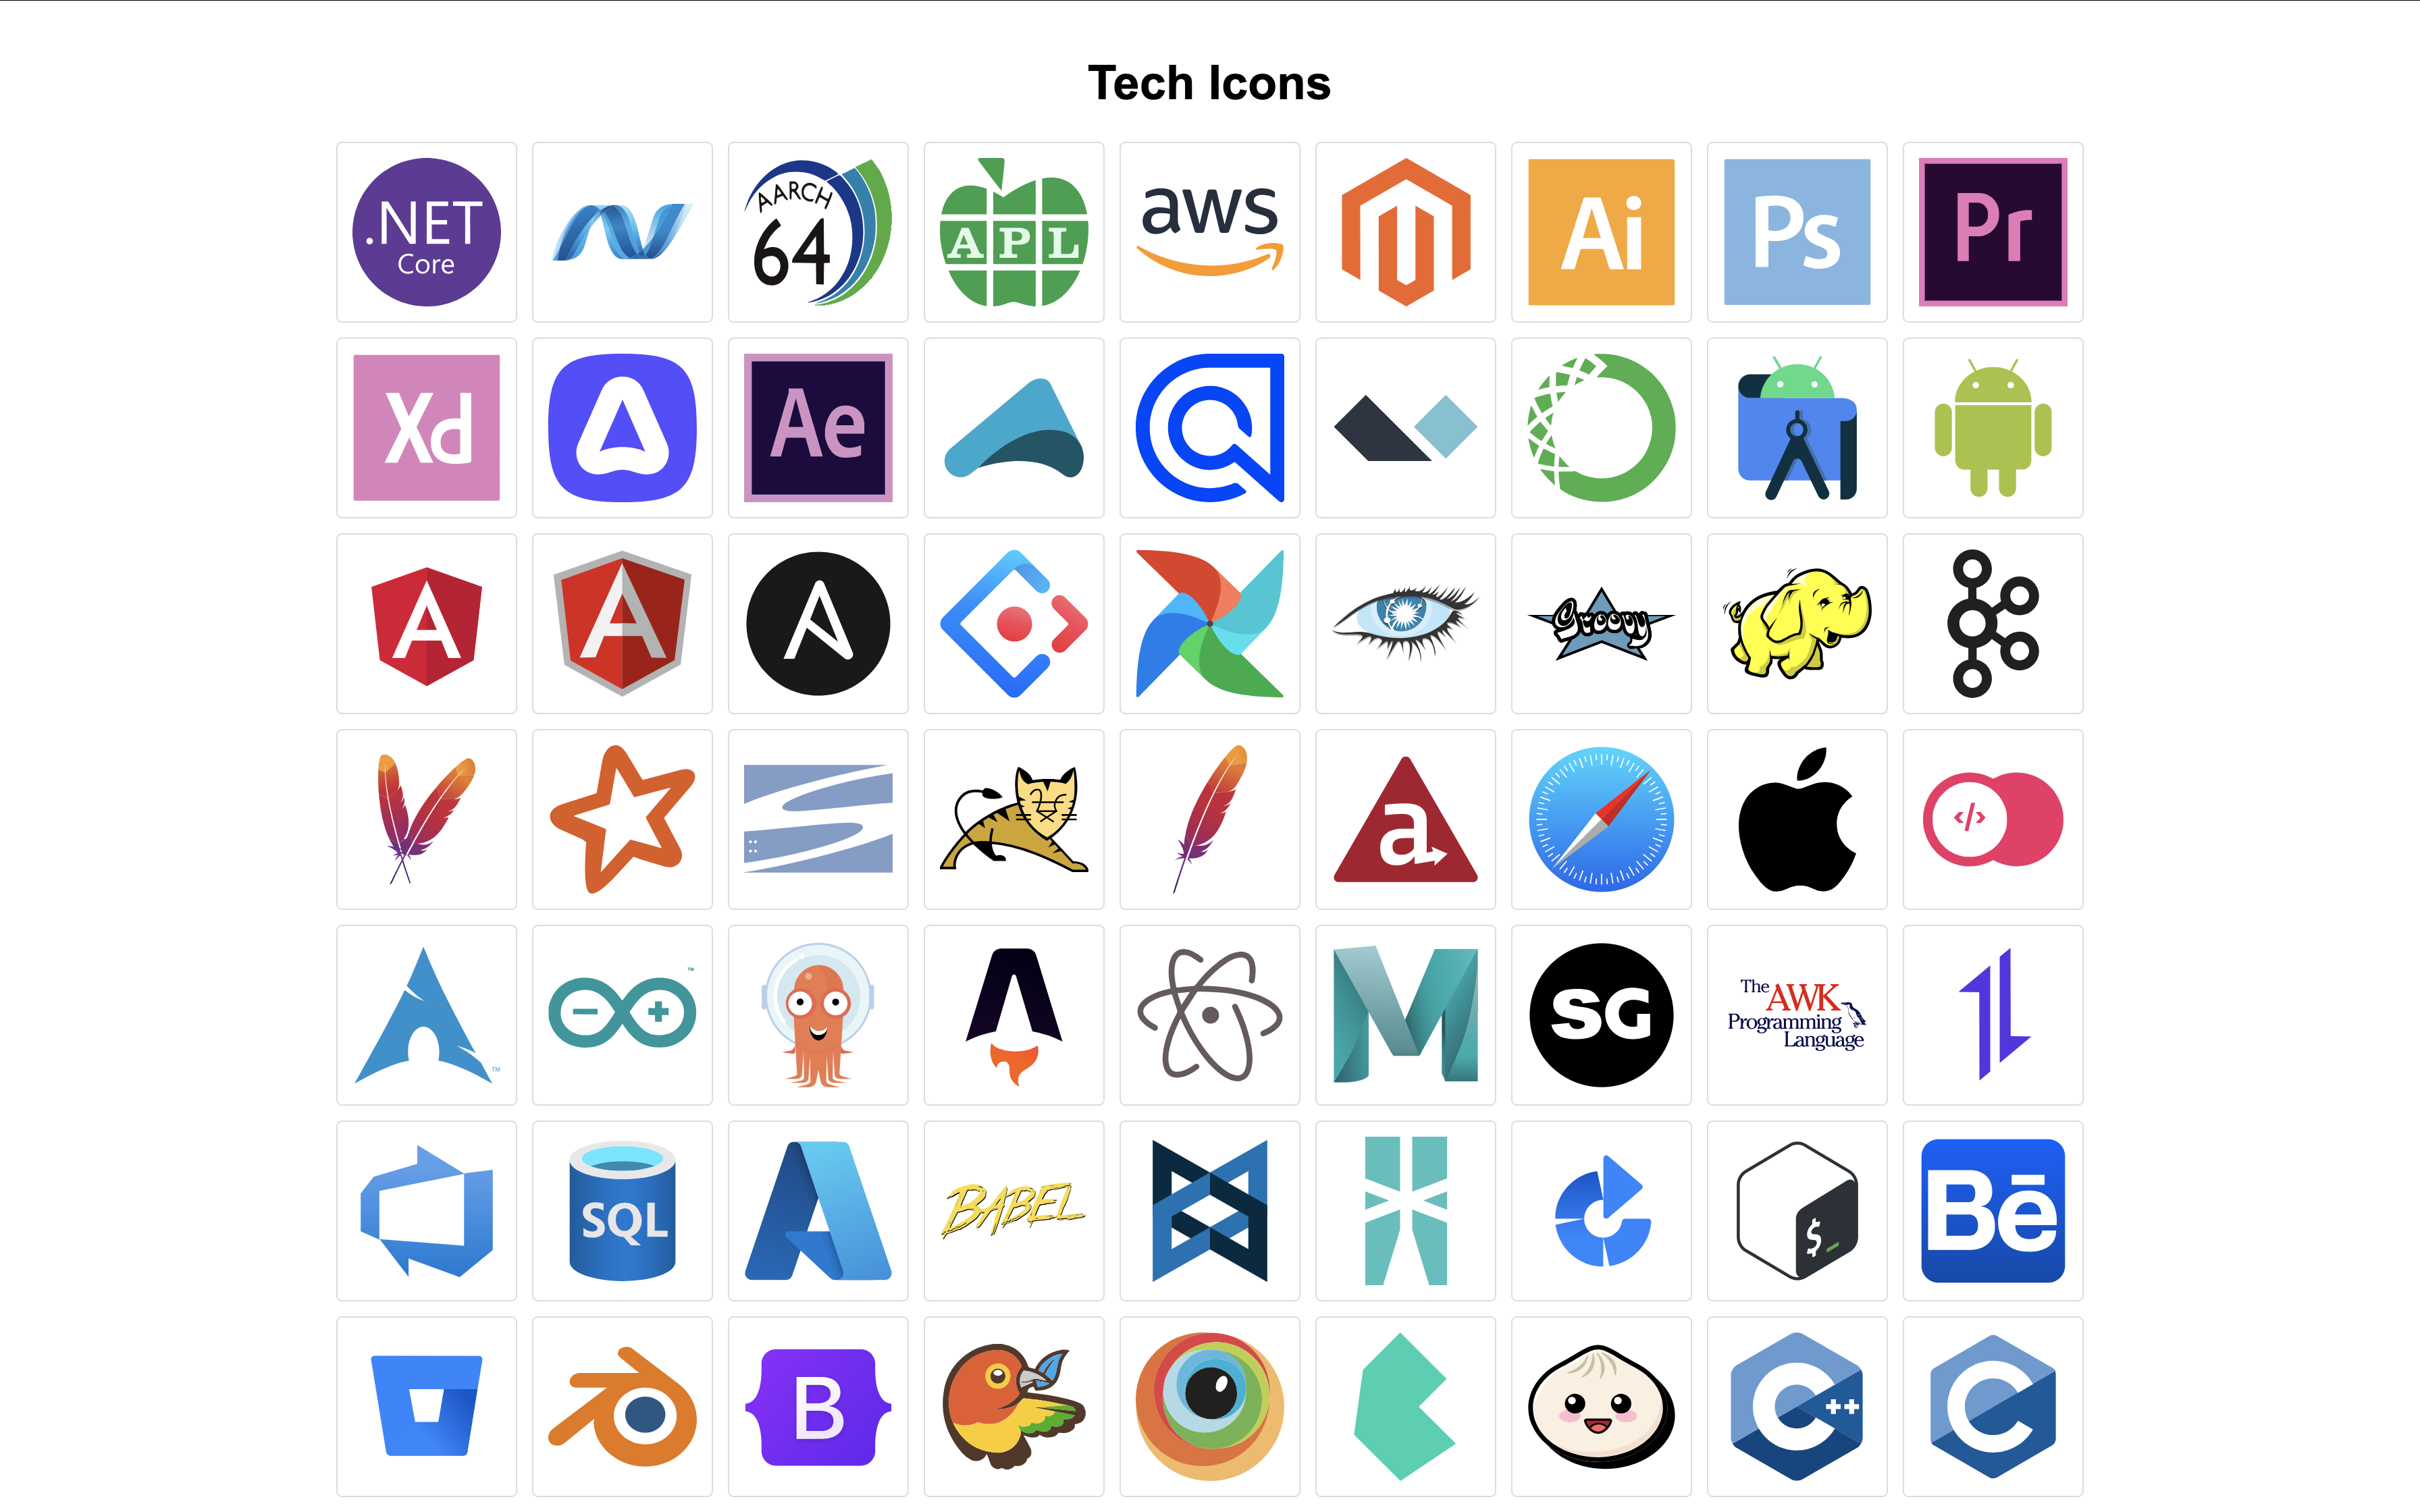
\includegraphics[width=.95\textwidth]{../assets/ci_reports_gcs_access/proxy-load-test.png}
    \caption{Result of retrieving the \texttt{index.html} file during the proxy load test}
    \label{fig:proxy-load-test}
\end{figure}

\section{Building and Deployment}

The proxy application is containerized using Docker and deployed through the existing GitHub Actions-based \acs{CI}/\acs{CD} infrastructure. This approach provides a reproducible build process and ensures that the same container image is used throughout the deployment process.

\subsection{Building the Docker Image}

A dedicated \texttt{Dockerfile} is used to package the application into a production-ready Docker image. Several optimization techniques are applied to reduce both the build time and the size of the final image:

\begin{itemize}
    \item \textbf{Dependency caching with pnpm:} The CI/CD environment uses the caching mechanism provided by \texttt{pnpm} to reuse previously downloaded dependencies. Instead of downloading all packages from the registry for every build, packages already available in the pnpm store can be reused, reducing network transfers and dependency installation time.

    \item \textbf{Distroless runtime image:} The runner stage is based on a \textbf{Distroless} Node.js image \texttt{gcr.io/distroless/nodejs24-debian12}. Distroless images contain only the components required to execute the application and omit unnecessary operating-system utilities, such as package managers, shells and other command-line tools. This reduces the final image size and attack surface while providing a lightweight production environment.

    \item \textbf{Docker layer caching:} The \texttt{package.json} and \texttt{pnpm-lock.yaml} files are copied before the application source code. This allows Docker to reuse the dependency installation layer as long as the project's dependencies have not changed. Consequently, modifications to the application source code do not trigger a complete reinstallation of \texttt{node\_modules}.
\end{itemize}

These optimization techniques result in a smaller production image and a faster, more efficient CI/CD build process while maintaining a reproducible application build.

The Dockerfile used for the application is illustrated below:

\begin{lstlisting}[language=Docker, caption={Dockerfile for the production image}, label={lst:gcs-proxy-dockerfile}]
FROM gcr.io/distroless/nodejs24-debian12:nonroot AS runner

ENV PORT=3000 \
    NODE_ENV=production

# Only needed for local development.
ENV NODE_TLS_REJECT_UNAUTHORIZED=0

WORKDIR /app

COPY --chown=nonroot:nonroot package.json pnpm-lock.yaml .npmrc .env ./
COPY --chown=nonroot:nonroot node_modules ./node_modules
COPY --chown=nonroot:nonroot public ./public
COPY --chown=nonroot:nonroot dist ./dist

EXPOSE 3000

CMD ["/app/dist/index.js"]
\end{lstlisting}

\subsection{Deployment}

The build and deployment process is integrated into the project's GitHub Actions workflow. When the application is built, the workflow uses the Dockerfile to generate the production image and publishes it to the organization's container registry. The resulting image is then used to deploy the application to the \textbf{Dev8} environment.

The deployment process can be summarized as follows:

\begin{enumerate}

    \item The application source code is checked out by the GitHub Actions workflow.

    \item The project dependencies are installed and the application is built in the CI/CD environment.

    \item The Docker image is built using the project's \texttt{Dockerfile}. The build process reuses the dependencies installed in the CI/CD environment and copies the required application artifacts, including \texttt{node\_modules}, \texttt{dist}, and \texttt{public}, from the GitHub Actions runner into the Docker image.

    \item The generated Docker image is tagged with a version identifier and published to the internal container registry.

    \item The Dev8 deployment process retrieves the published image from the container registry.

    \item The application is started in a container using the newly deployed image and the configuration provided by the infrastructure environment.

    \item Consul verifies the availability of the deployed service by periodically querying the application's health-check endpoint. If the service responds with a healthy status, the deployment is considered operational.

\end{enumerate}

A dedicated GitHub Action provided by the internal \texttt{shared-actions} repository is used to version the Docker image according to \ac{SemVer} (\textit{Semantic Versioning}) rules. This ensures that each published image receives a consistent and meaningful version identifier based on the changes introduced in the application.

The generated version is used as the Docker image tag and associates the deployed container image with a specific version of the source code. This provides traceability throughout the deployment lifecycle and makes it possible to identify and reproduce the exact application version deployed to the Dev8 environment.

\subsection{Environment Configuration and Secrets}

The application requires several environment variables to configure its runtime behavior, including the credentials and configuration required to access Google Cloud Storage. These values are not stored directly in the source code or Docker image.

Instead, the required environment variables are defined in the repository's \texttt{config-unified} in an encrypted form. This configuration provides a centralized mechanism for managing environment-specific values while preventing sensitive information from being exposed in the repository.

The decryption and injection of these values are handled by the \textbf{Infrastructure team}. During deployment, the infrastructure layer retrieves and decrypts the required configuration, then passes the resulting environment variables to the running application.

Consequently, sensitive configuration remains separated from both the application source code and the Docker image. The application only receives the required values at runtime, while the infrastructure team remains responsible for their secure storage, decryption and injection.

\subsection{Deployment to Dev8}

The application is deployed to the \textbf{Dev8} environment after its Docker image has been successfully published. The infrastructure deployment mechanism retrieves the corresponding image from the container registry and starts the application with the appropriate Dev8 configuration.

The deployment architecture separates application concerns from infrastructure concerns. The development team is responsible for the application code, Docker image and CI workflow, while the Infrastructure team manages the deployment environment, secrets, environment variables and the mechanisms used to securely inject them into the application.

After deployment, the application's \texttt{/health} endpoint is monitored by \textbf{Consul}, the service discovery and health-check tool used within the infrastructure. Consul periodically sends requests to this endpoint to verify that the service is operational and responding correctly. This integrates the deployment process with the health-check and monitoring mechanisms described previously, allowing the infrastructure to detect service failures and react accordingly.

\section{Back to VRT Infrastructure}

Once the proxy application has been successfully deployed and its availability has been verified, a few minor modifications are made to the existing \ac{VRT} infrastructure. The objective is to integrate the newly deployed proxy into the existing workflow without changing the overall report generation and publication process.

The \ac{VRT} workflow is updated to replace direct references to the private \ac{GCS} URLs with the corresponding proxy URLs and endpoints. As a result, subsequent requests to access, verify, search, or download \ac{VRT} reports are routed through the proxy rather than directly to \ac{GCS}.

This modification allows the \ac{VRT} infrastructure to benefit from the proxy's authentication and access mechanisms while keeping the underlying \ac{GCS} buckets private. It also avoids requiring the \ac{VRT} workflow or end users to handle Google Cloud authentication directly.

\textbf{Note:} GitHub applies URL sanitization mechanisms that prevent images served through the proxy application from being rendered correctly (Because the proxy application is only accessible from within the Rakuten infrastructure). As a temporary workaround, time-limited \ac{GCS} URLs with a validity period of 7 days are used for images embedded in \ac{VRT} reports. This approach preserves the ability to display the images while limiting the exposure period of the underlying resources.

\section{Conclusion}

The developed proxy provides secure and efficient access to \ac{CI} artifacts stored in private \ac{GCS} buckets. By combining authenticated access, token caching, streaming, a simple web interface and monitoring endpoints, the application improves report accessibility while preserving the security of the underlying storage infrastructure. Furthermore, the project provided valuable experience covering the complete software engineering lifecycle, from requirements analysis and architecture design to implementation, testing and deployment.

\clearpage
